%!TEX root = ../mst.tex

\chapter{Introduction}
A \textbf{homogeneous system} is a system in which chemical and physical
properties are independent of the position (uniform).

a \textbf{heterogeneous system} is a system in which chemical and physical
properties depend on the position. A particular set of heterogeneous systems are
multiphase systems.

A \textbf{multiphase system} can be thought as a heterogeneous system coming
from the union of homogeneous systems. Each homogeneous portion is called
\textbf{phase}.

\begin{figure}[htp]
    \centering
    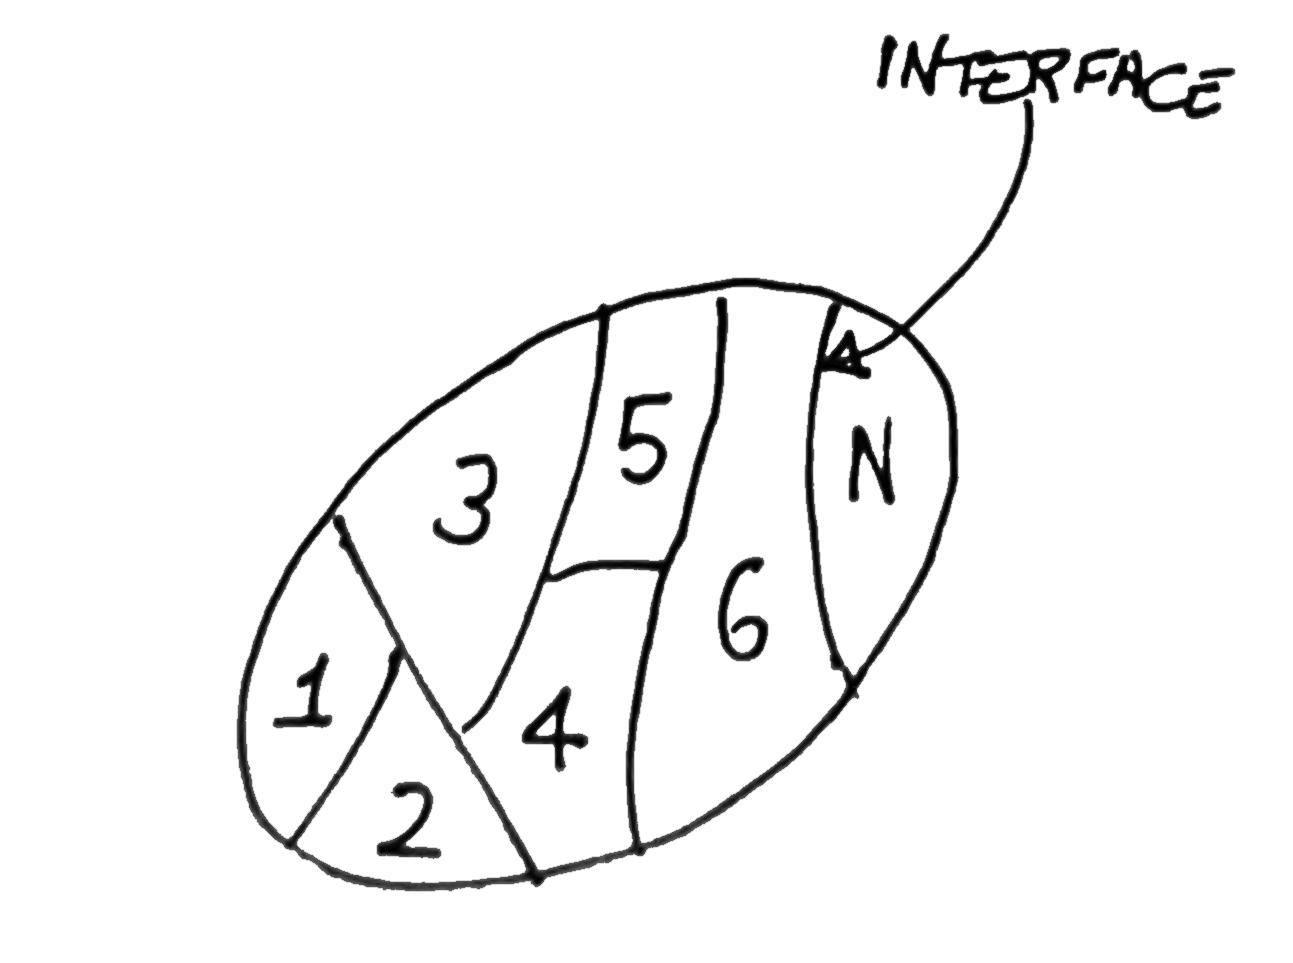
\includegraphics[width=.3\textwidth]{multiphase_system}
    \caption{A multiphase system.}
\end{figure}

Phases are separated by boundaries, called \textbf{interfaces}. Interface are
usually:
\begin{itemize}
    \item deformable (moving);
    \item diathermal (diabatic);
    \item permeable to chemical species.
\end{itemize}

From the point of view of energy, an interface usually allows the exchange of
work, heat and chemical energy.

\section{Thermodynamic equilibrium}
\subsection{How many phases can coexist at equilibrium?}
Let's consider a system with $M$ phases and $r$ chemical components (chemical
species). Then let's write equilibrium equations:
\begin{itemize}
    \item \textbf{Mechanical equilibrium}: for planar interfaces\footnote{The
    number of equations is independent of the shape of the interface, but for
    the sake of simplicity we will consider flat boundaries. We will extend
    these considerations when dealing with bubbles or drops.} pressure $p$ is
    uniform
    \begin{equation*}
        p^{(1)} = p^{(2)} = \dots = p^{(M)}
    \end{equation*}
    \item \textbf{Thermal equilibrium}: temperature $T$ is uniform
    \begin{equation*}
        T^{(1)} = T^{(2)} = \dots = T^{(M)}
    \end{equation*}
    \item \textbf{Chemical equilibrium}: we have $r\times M$ equations, chemical
    potential is the same throughout the heterogeneous system
    \begin{align*}
        \mu_1^{(1)} &= \mu_1^{(2)} = \dots = \mu_1^{(M)} \\
        \mu_2^{(1)} &= \mu_2^{(2)} = \dots = \mu_2^{(M)} \\
        &\vdots \\
        \mu_r^{(1)} &= \mu_r^{(2)} = \dots = \mu_r^{(M)}
    \end{align*}
\end{itemize}

This system of equations states the thermodynamic equilibrium and contains
$M\times(r+2)$ variables and $(M-1)\times(r+2)$ equations.

Each one of the $M$ phases is an homogeneous system by itself, hence each phase
has to satisfy the Gibbs-Duhem Equation to fullfill the first and second
principles of thermodynamics:
\begin{equation*}
    SdT-Vdp+\sum_{i=1}^r N_id\mu_i = 0
\end{equation*}
The real number of equations now becomes $(M-1)\times(r+2) + M$.

Given that the well-posedness of a system arises when $\#\text{ Variables} \ge
\#\text{ Equations}$,
\begin{align*}
    \#\text{ Equations} &\le \#\text{ Variables} \\
    (M-1)(r+2)+M &\le M(r+2) \\
    M(r+2)-r-2+M &\le M(r+2) \\
    M &\le r+2
\end{align*}

\subsubsection{Examples}
In the case $r=1$ (single component system),
\begin{equation*}
    r=1 \implies M \le 3 \quad
    \begin{cases}
        M = 3 \to \text{ three phase system (triple state)} \\
        M = 2 \to \text{ two phase system} \\
        M = 1 \to \text{ single phase system}
    \end{cases}
\end{equation*}

In the case $r=2$ (two component system), $r=2 \implies M \le 4$. An example
could be moist air, given that we approximate dry air as if it was made by a
single component. In a lab environment could be possible to observe a mixture of
condensed air, condensed water and moist air.

\subsection{How many quantities are required to describe equilibrium?}
Let’s now derive the number of indipendent variables (also known as
\emph{degrees of freedom}):
\begin{align*}
    f &= \#\text{ Variables} - \#\text{ Equations} \\
    &= M(r+2) - (M-1)(r+2) - M \\
    &= M(r+2) - M(r+2) + r+2 - M \\
    &= r - M + 2
\end{align*}

\subsubsection{Examples}
For a single component system ($r=1$) the degrees of freedom are $f=3-M$. Three
cases:
\begin{itemize}
    \item $M=3 \to f=0$ meaning that we cannot set any quantity among
    temperature, pressure and chemical potential;
    \item $M=2 \to f=1$ meaning we are only allowed to set one variable,
    typically the temperature or the pressure (\emph{saturation condition});
    \item $M=1 \to f=2$ meaning we are free to set temperature and pressure
    independently.
\end{itemize}

\section{Basic quantities}
We start by considering two-phase gas-liquid\footnote{Two components, $M \le
4$.} or vapour-liquid flows\footnote{One component, $M \le 3$.}. To study fluid
dynamics of a single phase system we can write EDPs that are able to give the
distribution of all the quantities related to the flow field at any point inside
the pipeline.

In the case of more than one phase flowing in a pipe, no analytical solutions
are available, and moreover the numerical methods effective for single phase
flows fail to properly simulate all the relevant quantity.

For design purposes, we need a simplified approach and hence we will adopt a
\emph{one-dimentional axial flow model} that lumps the information pertaining
the distribution of the velocity of the phases using cross section averages. We
are only interested in determining the behaviour of the relevant quantities
along the pipe axis.

\subsection{Total Volume Flow Rate}
Volume Flow Rate is the rate at which volume flows in the pipe. Its unit is
$[\si{\cubic\metre\per\second}]$ in SI units.
\begin{equation}
    Q = Q_g + Q_l
    \label{eq:total_volume_flow_rate}
\end{equation}
where subscript $g$ stands for \emph{gas} whereas $l$ stands for \emph{liquid}.

\subsection{Average Volume Quality}
Based on the definition of Total Volume Flow Rate we can define a quantity
related to phase fractions. If we divide each member of
Eq.~\ref{eq:total_volume_flow_rate} by Q,
\begin{equation*}
    1 = \frac{Q_g}{Q} + \frac{Q_l}{Q}
\end{equation*}

We now define $\overline{x_v}$ (cross-section average) as follows:
\begin{equation*}
    \overline{x_v} = \frac{Q_g}{Q}
\end{equation*}
Average Volume Quality is adimensional.

\subsection{Total Mass Flow Rate}
If we call the phase densities $\rho_g$ and $\rho_l$ (in SI units
$[\si{\kg\per\cubic\metre}]$) we can also define Mass Flow Rates: $\Gamma_g =
\rho_gQ_g$ for the gas and $\Gamma_l = \rho_lQ_l$ for the liquid.

Since mass is additive, we can write the Total Mass Flow Rate (in SI units
$[\si{\kg\per\s}]$):
\begin{equation}
    \Gamma = \Gamma_g + \Gamma_l
    \label{eq:total_mass_flow_rate}
\end{equation}

Recall that instead of phase densities we can use their reciprocal,
\emph{specific volumes}:
\begin{align*}
    v_g &= \frac{1}{\rho_g} \\
    v_l &= \frac{1}{\rho_l}
\end{align*}

\subsection{Average Mass Quality}
Dividing each member of Eq.~\ref{eq:total_mass_flow_rate} by $\Gamma$:
\begin{equation*}
    1 = \frac{\Gamma_g}{\Gamma} + \frac{\Gamma_l}{\Gamma}
\end{equation*}

We define $\overline{x}$, the Average Mass Quality:
\begin{equation*}
    \overline{x} = \frac{\Gamma_g}{\Gamma}
\end{equation*}
Mass quality is adimensional.

\subsection{Relationship between $\overline{x}$ and $\overline{x_v}$} Owing to
the difference in densities (or specific volumes), the numerical values of mass
quality $\overline{x}$ and volume quality $\overline{x_v}$ may differ greatly.

Starting from volume quality,
\begin{align*}
    \overline{x_v} &= \frac{Q_g}{Q} = \frac{Q_g}{Q_g+Q_l} = \frac{1}{1+\frac{\textcolor{Blue}{Q_l}}{\textcolor{BrickRed}{Q_g}}} = \\
    &= \frac{1}{1+\textcolor{Blue}{\frac{\Gamma_l}{\rho_l}}\textcolor{BrickRed}{\frac{\rho_g}{\Gamma_g}}} = \\
    &= \frac{1}{1+\frac{\rho_g}{\rho_l}\frac{(1-\overline{x})\cancel{\Gamma}}{\overline{x}\cancel{\Gamma}}}
\end{align*}

In a more elegant form:
\begin{equation*}
    \frac{1-\overline{x_v}}{\overline{x_v}} = \frac{\rho_g}{\rho_l}\frac{1-\overline{x}}{\overline{x}}
\end{equation*}

Generally $\rho_g \ll \rho_l$, hence $\overline{x_v} \gg \overline{x}$. For a
pure liquid-vapour mixture $\rho_g-\rho_l$ lowers with $T$ (or $p$) and at a
critical point $\rho_g=\rho_l$.

\begin{figure}[htp]
    \centering
    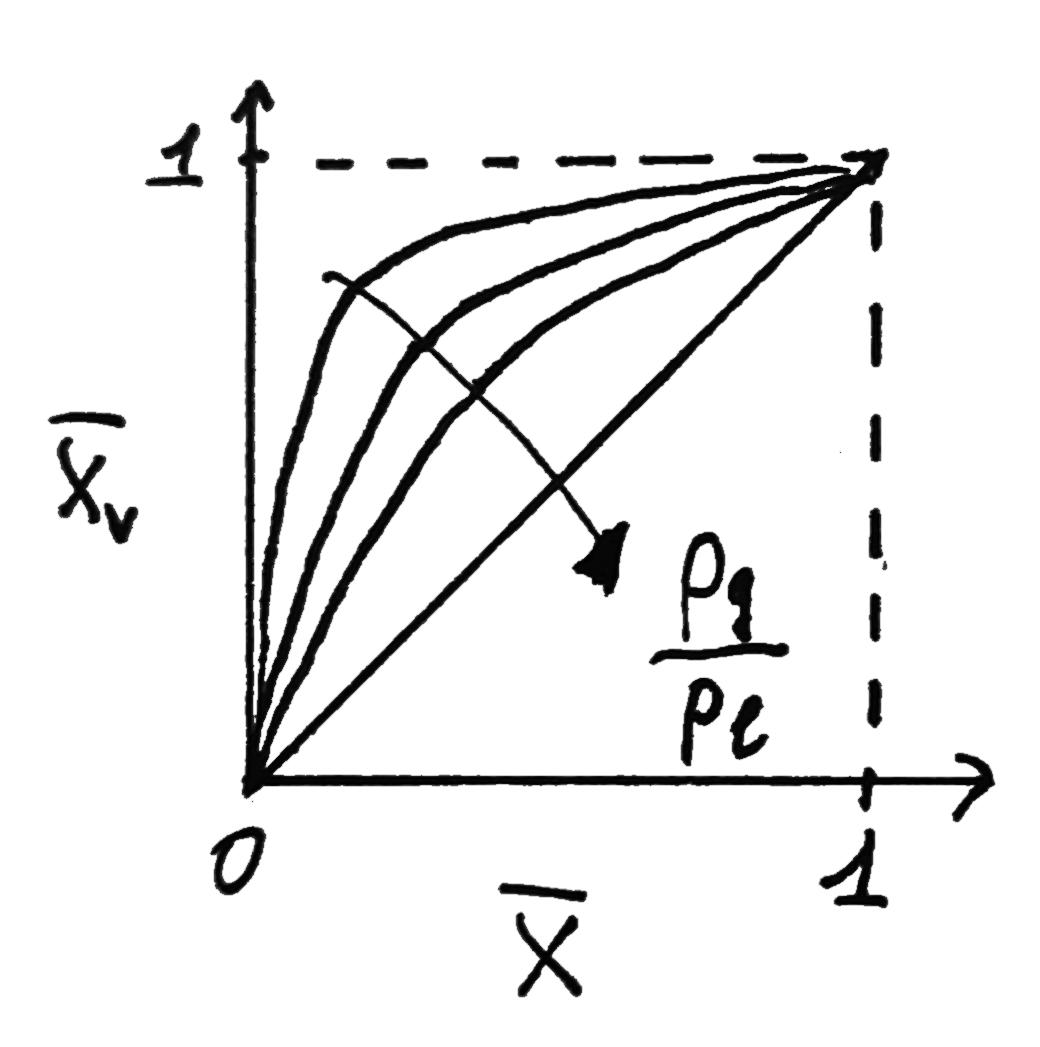
\includegraphics[width=.25\textwidth]{avg_x_v_vs_x_v}
    \caption{Volume Quality vs Mass Quality.}
\end{figure}

\subsection{Bulk Density}
The ratio between the mass flow rate and the volume flow rate has the dimensions
of a density and is called bulk density. It is the density that would pertain to
an equivalent single-phase fluid flowing with the same mass and volume flow
rates of the two-phase mixture.

Referring to the cross-section average, the bulk density $\overline{\rho_b}$ is
such that:
\begin{equation*}
    \overline{\rho_b} = \frac{\Gamma}{Q}
\end{equation*}

Let's specialize the numerator in the previous equation:
\begin{equation*}
    \overline{\rho_b} = \frac{\Gamma_g + \Gamma_l}{Q} = \frac{\rho_gQ_g + \rho_lQ_l}{Q} = \rho_g\overline{x_v}+\rho_l(1-\overline{x_v})
\end{equation*}

On the other hand, we can specialize the denominator:
\begin{equation*}
    \overline{\rho_b} = \frac{\Gamma}{Q_g+Q_l} = \frac{\Gamma}{v_g\Gamma_g+v_l\Gamma_l} = \frac{1}{v_g\overline{x}+v_l(1-\overline{x})} = \frac{1}{\overline{v_b}}
\end{equation*}
where $\overline{v_b}$ is the \emph{bulk specific volume}.

Bulk density and bulk specific volume are only apparent quantities of the
flowing mixture and cannot be considered if we're interested in the real mass or
volume content in the pipeline. This is because the two phases do not travel
with the same velocities (phase slippage).

% lecture 2 min 28